%!TEX program = xelatex

\documentclass[a4paper, openany, oneside]{memoir}
\usepackage[no-math]{fontspec}
\usepackage{pgfplots}
\pgfplotsset{compat=newest}
\usepackage{commath}
\usepackage{mathtools}
\usepackage{amssymb}
\usepackage{amsthm}
\usepackage{booktabs}
\usepackage{mathtools}
\usepackage{xcolor}
\usepackage[separate-uncertainty=true, per-mode=symbol]{siunitx}
\usepackage[noabbrev, capitalize]{cleveref}
\usepackage{listings}
\usepackage[american inductor, european resistor]{circuitikz}
\usepackage{amsmath}
\usepackage{amsfonts}
\usepackage{ifxetex}
\usepackage[dutch,english]{babel}
\usepackage[backend=bibtexu,texencoding=utf8,bibencoding=utf8,style=ieee,sortlocale=en_GB,language=auto]{biblatex}
\usepackage[strict,autostyle]{csquotes}
\usepackage{parskip}
\usepackage{import}
\usepackage{standalone}
\usepackage{hyperref}
%\usepackage[toc,title,titletoc]{appendix}

\ifxetex{} % Fonts laden in het geval dat je met Xetex compiled
    \usepackage{fontspec}
    \defaultfontfeatures{Ligatures=TeX} % To support LaTeX quoting style
    \setromanfont{Palatino Linotype} % Tover ergens in Font mapje in root.
    \setmonofont{Source Code Pro}
\else % Terug val in standaard pdflatex tool chain. Geen ondersteuning voor OTT fonts
    \usepackage[T1]{fontenc}
    \usepackage[utf8]{inputenc}
\fi
\newcommand{\references}[1]{\begin{flushright}{#1}\end{flushright}}
\renewcommand{\vec}[1]{\boldsymbol{\mathbf{#1}}}
\newcommand{\uvec}[1]{\boldsymbol{\hat{\vec{#1}}}}
\newcommand{\mat}[1]{\boldsymbol{\mathbf{#1}}}
\newcommand{\fasor}[1]{\boldsymbol{\tilde{\vec{#1}}}}
\newcommand{\cmplx}[0]{\mathrm{j}}
\renewcommand{\Re}[0]{\operatorname{Re}}
\newcommand{\Cov}{\operatorname{Cov}}
\newcommand{\Var}{\operatorname{Var}}
\newcommand{\proj}{\operatorname{proj}}
\newcommand{\Perp}{\operatorname{perp}}
\newcommand{\col}{\operatorname{col}}
\newcommand{\rect}{\operatorname{rect}}
\newcommand{\sinc}{\operatorname{sinc}}
\newcommand{\IT}{\operatorname{IT}}
\newcommand{\F}{\mathcal{F}}

\newtheorem{definition}{Definition}
\newtheorem{theorem}{Theorem}


\DeclareSIUnit{\voltampere}{VA} %apparent power
\DeclareSIUnit{\pii}{\ensuremath{\pi}}

\hypersetup{%setup hyperlinks
    colorlinks,
    citecolor=black,
    filecolor=black,
    linkcolor=black,
    urlcolor=black
}

% Example boxes
\usepackage{fancybox}
\usepackage{framed}
\usepackage{adjustbox}
\newenvironment{simpages}%
{\AtBeginEnvironment{itemize}{\parskip=0pt\parsep=0pt\partopsep=0pt}
\def\FrameCommand{\fboxsep=.5\FrameSep\shadowbox}\MakeFramed{\FrameRestore}}%
{\endMakeFramed}

% Impulse train
\DeclareFontFamily{U}{wncy}{}
\DeclareFontShape{U}{wncy}{m}{n}{<->wncyr10}{}
\DeclareSymbolFont{mcy}{U}{wncy}{m}{n}
\DeclareMathSymbol{\Sha}{\mathord}{mcy}{"58}
\addbibresource{../../../includes/bibliography.bib}

\title{Compressive Sensing - An Overview}

\author{W.P. Bruinsma \and R.P. Hes \and H.J.C. Kroep \and T.C. Leliveld \and W.M. Melching \and T.A. aan de Wiel}

\raggedbottom

\begin{document}
\chapter{Jammer}
\label{cha:jammer}

\subsection{Introduction}
For our business plan we considered building a smart jammer. When the signals that are present in the spectrum are identified a list of frequencies that need to be jammed can be generated. To do the actual jamming we decided to build a simple device to block one programmable frequency. The number of transmitters should scale with the number of expected signals in the frequency range that needs to be jammed.

In this section we will discuss the working of this jammer. We will begin with a block diagram of the transmitter, and we will then present the complete schematics and the PCB\@. Unfortunately, because this was a small side project, we did not have enough time to actually finish the design and build it.

\begin{figure}[H]
\centering
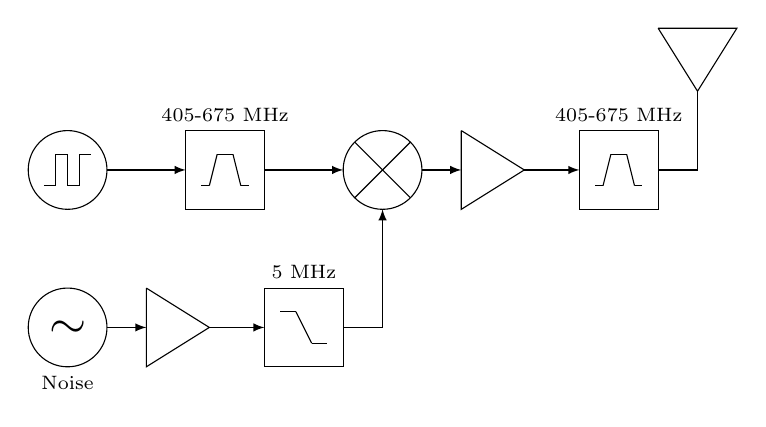
\begin{tikzpicture}

\draw [>=latex, ->] (-0.5,6) -- (0.5,6);
\draw [>=latex, ->] (3.5,6) -- (4,6);
\draw [>=latex, ->] (-0.5,4) -- (0,4);
\draw [>=latex, ->] (0.8,4) -- (1.5,4);
\draw [>=latex, ->] (4.8,6) -- (5.5,6);

\draw [>=latex, ->] (3,4) -- (3,5.5);
\draw (2.5,4) -- (3,4);

\draw (7,6) -- (7,7);
\draw (6.5,6) -- (7,6);

\draw (6.5,7.8) -- (7,7) -- (7.5,7.8) -- (6.5,7.8);

\draw (0.5,6.5) rectangle (1.5,5.5) node[pos=.5]{};
\draw (0.7,5.8) -- (0.8,5.8);
\draw (1.2,5.8) -- (1.3,5.8);
\draw (0.8,5.8) -- (0.9,6.2);
\draw (1.2,5.8) -- (1.1,6.2);
\draw (0.9,6.2) -- (1.1,6.2);

\draw (5.5,6.5) rectangle (6.5,5.5) node[pos=.5]{};
\draw (5.7,5.8) -- (5.8,5.8);
\draw (6.2,5.8) -- (6.3,5.8);
\draw (5.8,5.8) -- (5.9,6.2);
\draw (6.2,5.8) -- (6.1,6.2);
\draw (5.9,6.2) -- (6.1,6.2);

\draw (0,4.5) -- (0.8,4) -- (0,3.5) -- (0,4.5);
\draw (4,6.5) -- (4.8,6) -- (4,5.5) -- (4,6.5);


\draw (1.5,4.5) rectangle (2.5,3.5) node[pos=.5]{};

\draw (2.1,3.8) -- (2.3,3.8);
\draw (2.1,3.8) -- (1.9,4.2);
\draw (1.7,4.2) -- (1.9,4.2);
\draw [>=latex, ->] (1.5,6) -- (2.5,6);

\draw  (-1,6) ellipse (.5 and .5) node{};
\draw (-1.3,5.8) -- (-1.15,5.8);
\draw (-1.15,6.2) -- (-1.15,5.8);
\draw (-1.15,6.2) -- (-1,6.2);
\draw (-1,5.8) -- (-0.85,5.8);
\draw (-1,6.2) -- (-1,5.8);
\draw (-0.85,6.2) -- (-0.7,6.2);
\draw (-0.85,6.2) -- (-0.85,5.8);

\draw  (-1,4) ellipse (.5 and .5);
\node at (-1,3.97) {\LARGE$\sim$};

\draw  (3,6) ellipse (.5 and .5) node{};
\draw (2.65,5.65) -- (3.35,6.35);
\draw (2.65,6.35) -- (3.35,5.65);

\node at (1,6.7) {\scriptsize 405-675 MHz};
\node at (6,6.7) {\scriptsize 405-675 MHz};
\node at (2,4.7) {\scriptsize 5 MHz};
\node at (-1,3.3) {\scriptsize Noise};
\end{tikzpicture}
\caption{Block diagram of the jammer}
\label{fig:block_diagram_jammer}
\end{figure}



The block diagram of the jammer can be found in \cref{fig:block_diagram_jammer}. The jammer works by generation a square wave with a programmable clock generator IC\@. These ICs are much cheaper than a solution with a very broadband voltage controller oscillator and a PLL\@. We chose a specific IC with a frequency range of \SIrange{3}{416}{\mega\hertz}. In this example we want to jam the band including the \SI{446}{\mega\hertz} frequency of licence free radios. Our oscillator only operates up to a frequency of \SI{416}{\mega\hertz}, therefore we need to select a high harmonic, in this case the third, and filter all of the other components of the square wave. In this case we use a bandpass filter that spans the \SIrange{405}{675}{\mega\hertz}. The bandwidth is determined by the frequency of the fifth harmonic. At \SI{405}{\mega\hertz} the base frequency is \SI{135}{\mega\hertz}, and the fifth harmonic \SI{675}{\mega\hertz}. We created a small script to generate a complete table of needed filters to span the whole range of \SI{3}{\mega\hertz} to \SI{3}{\giga\hertz}. These results can be found in \cref{tab:filter_freqs}.

After that the filtered signal is mixed with a band-limited noise source, and then amplified and filtered again. This should produce a band limited signal with noise at the desired frequency.

\begin{table}[h]
\centering
\caption{Filter frequencies for frequency range of \SIrange{3}{3179}{\mega\hertz}}
\label{tab:filter_freqs}
\begin{tabular}{rrrrr}
\toprule
   Harmonic &   Filter low [\si{\mega\hertz}] &   Filer high [\si{\mega\hertz}] &   LO low [\si{\mega\hertz}] &   LO high [\si{\mega\hertz}] \\
\midrule
          1 &            3 &            9 &        3 &         9 \\
          1 &            9 &           27 &        9 &        27 \\
          1 &           27 &           81 &       27 &        81 \\
          1 &           81 &          243 &       81 &       243 \\
          3 &          243 &          405 &       81 &       135 \\
          3 &          405 &          675 &      135 &       225 \\
          3 &          675 &         1125 &      225 &       375 \\
          5 &         1125 &         1575 &      225 &       315 \\
          7 &         1575 &         2025 &      225 &       289 \\
          7 &         2025 &         2601 &      289 &       371 \\
          9 &         2601 &         3179 &      289 &       353 \\
\bottomrule
\end{tabular}
\end{table}

\subsection{Schematics}
The schematics can be found in \cref{ap:jammer}.


\subsubsection{Filter design}
For this implementation we chose a frequency range of \SIrange{405}{675}{\mega\hertz}. We designed\footnote{Designed with \url{http://www-users.cs.york.ac.uk/~fisher/lcfilter/}} a sixth order Chebyshev bandpass filter, with a ripple of \SI{1.0}{\decibel} in the passband, a characteristic impedance of $50\,\Omega$. We also designed a matching network to match the $50\,\Omega$ of the filter to the $180\,\Omega$ input impedance of the mixer. The schematics of the filter can be found in \cref{fig:filter}.

\begin{figure}[h]
    \centering
    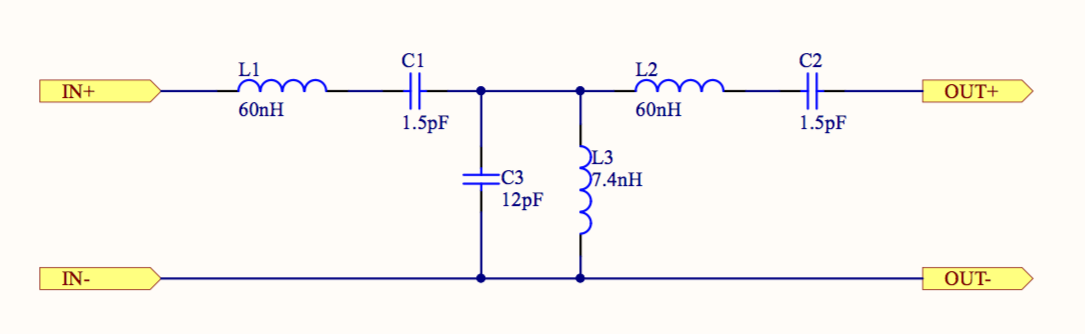
\includegraphics[width=\textwidth]{filter.png}
    \caption{The designed bandpass filter}
    \label{fig:filter}
\end{figure}

\subsubsection{Noise source}

\subsubsection{Microcontroller}
A microcontroller was needed to control the clock generator IC and communicate with the PC. We decided to use an Atmega 328P. This is the same microcontroller used as on the very widespread Arduino boards. Therefore a lot of code is already available. This would allow us to develop the firmware in the limited time we had left.

The microcontroller connects to the PC with a special FTDI usb to serial cable. With this setup we can easily send commands from our python program to the microcontroller.

\subsection{Simulations}
To verify the working of the system we built a SPICE simulation of a simplified version of the schematic. We also simulated the filters to check if those were designed correctly.

\subsubsection{Filters}
\begin{figure}[h]
    \centering
    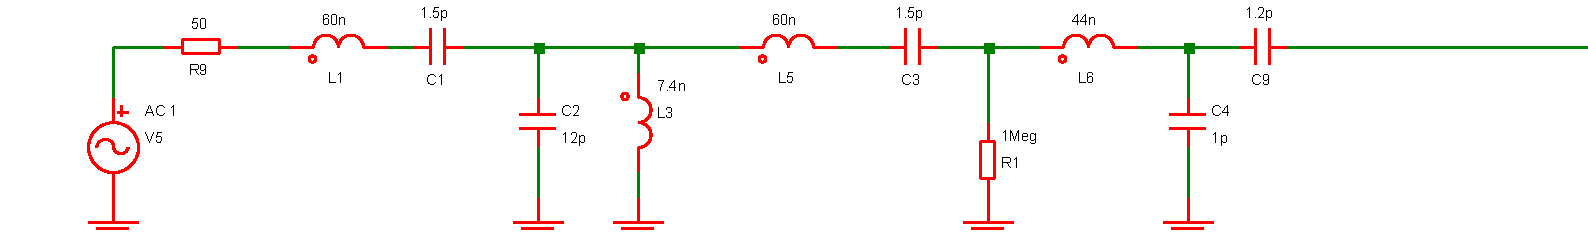
\includegraphics[width=\textwidth]{fig_sim_schematic.pdf}
    \caption{Schematic of the filter and matching network used in the simulation}
    \label{fig:sim_schematic}
\end{figure}

\begin{figure}[H]
\centering
\begin{tikzpicture}
\begin{axis}[
	xlabel={Frequency [\si{\hertz}]},
	ylabel={Gain [\si{\decibel}]},
	width=\textwidth, height=0.5\textwidth,
  xmode=log,
	ymax=10,
	ymin=-80,
  xmin=5e7,
  xmax=3e9,
	xmajorgrids, xminorgrids, ymajorgrids,
  name=gain
	]

%% Set the plot options, and load a csv formatted file %%
\addplot [
	color=black,
	solid,
	mark=.,
	]
	table [col sep=comma]{plots/gain_out.txt};
\end{axis}

\begin{axis}[
	xlabel={Frequency [\si{\hertz}]},
	ylabel={Phase [\si{\degree}]},
	width=\textwidth, height=0.5\textwidth,
  xmode=log,
	ymax=0,
	ymin=-720,
  xmin=5e7,
  xmax=3e9,
	xmajorgrids, xminorgrids, ymajorgrids,
  at=(gain.below south), anchor=above north
	]

%% Set the plot options, and load a csv formatted file %%
\addplot [
	color=black,
	solid,
	mark=.,
	]
	table [col sep=comma]{plots/phase_out.txt};
\end{axis}
\end{tikzpicture}
\caption{Bode plot of the designed filter and matching network}
\label{fig:plot_bode_filter}
\end{figure}

\subsubsection{Complete System}
We also did a simulation of the complete system, to check if our assumptions about the suppression of the unwanted harmonics worked correctly. We replaced the clock generator IC by a square wave source and the noise source by a theoretical noise source. The mixer was replaced by a theoretical multiplier. The resulting schematic can be found in \cref{fig:schematic_system_simulation}.

\begin{figure}[h]
    \centering
    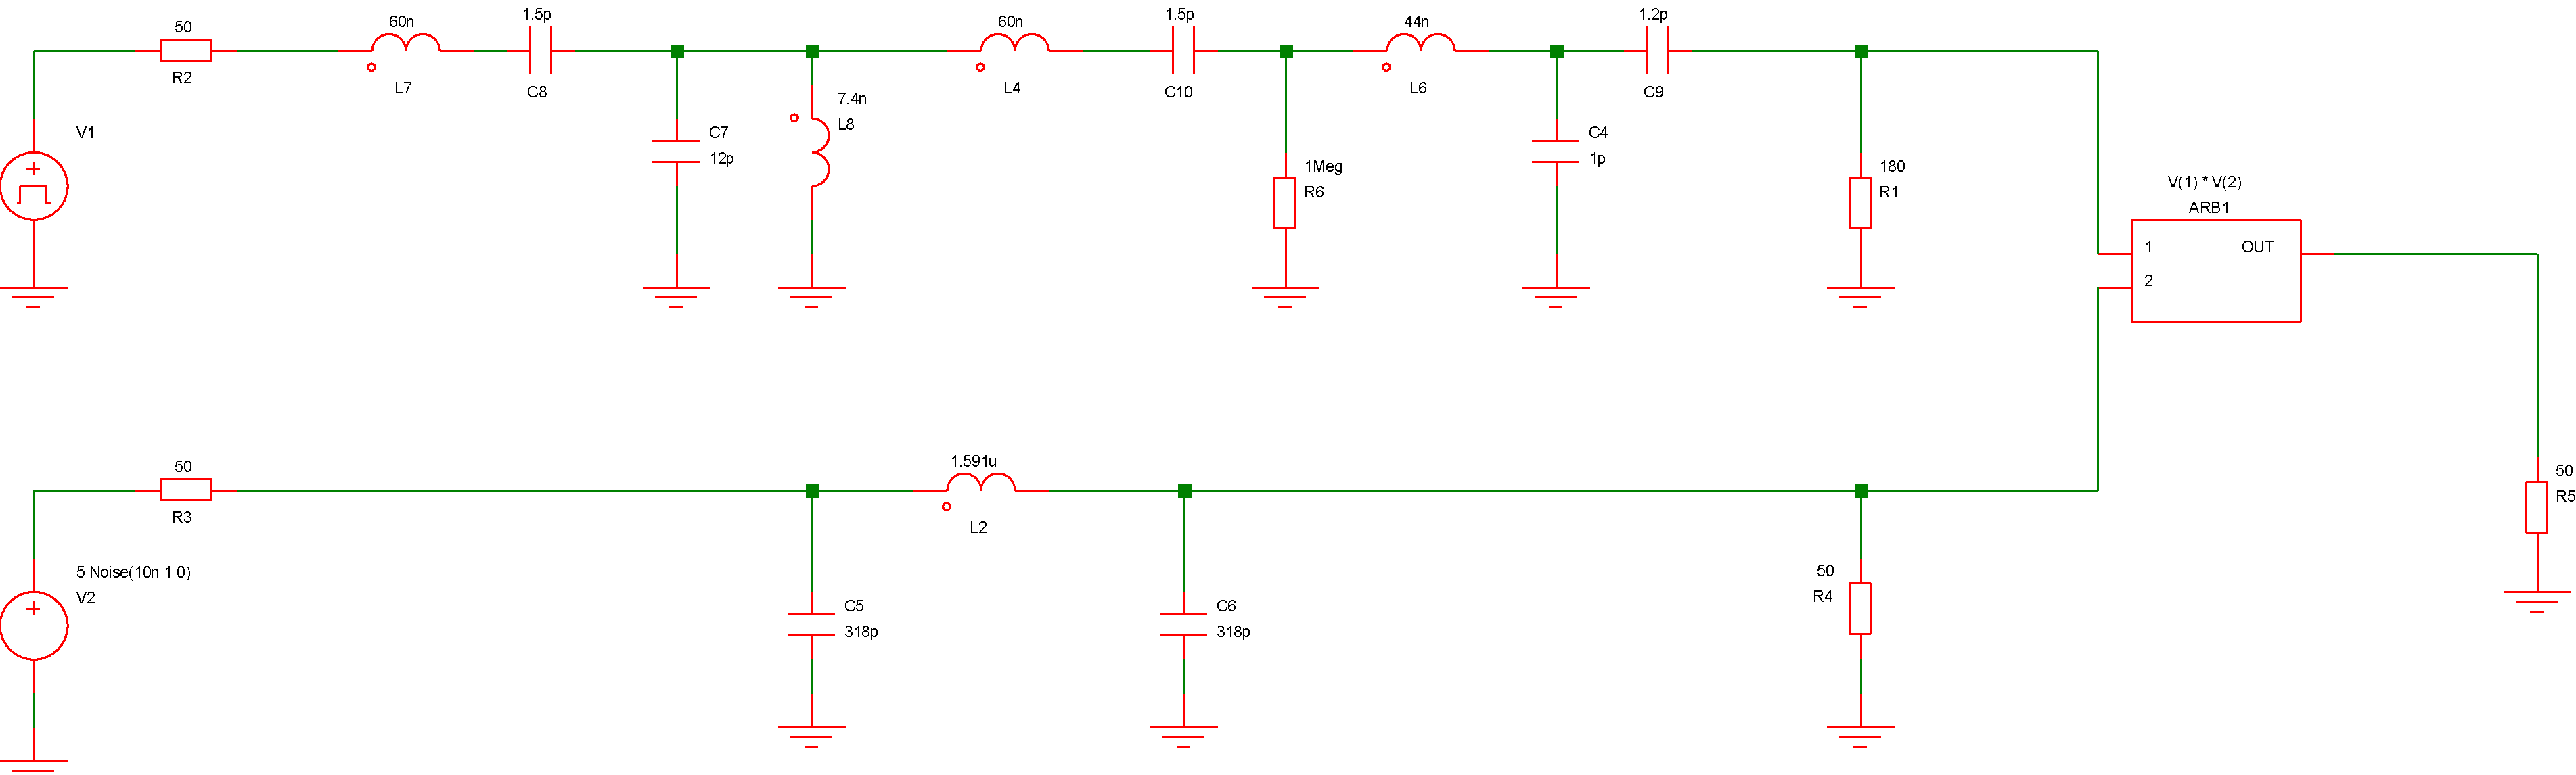
\includegraphics[width=\textwidth]{fig_sim_system_schematic.pdf}
    \caption{The schematic used for the system simulation}
    \label{fig:schematic_system_simulation}
\end{figure}


\begin{figure}[H]
\centering
\begin{tikzpicture}
\begin{axis}[
	xlabel={Frequency [\si{\hertz}]},
	ylabel={Spectrum [\si{\decibel}]},
	width=\textwidth, height=0.8\textwidth,
	ymax=-50,
	ymin=-200,
	xmajorgrids, xminorgrids, ymajorgrids,
	legend style={
		at={(0.02,0.97)},
		anchor=north west,
		legend cell align=left
		}
	]

%% Set the plot options, and load a csv formatted file %%
\addplot [
	color=black,
	solid,
	mark=.,
	]
	table [col sep=comma]{plots/system_out.txt};

\end{axis}
\end{tikzpicture}
\caption{Spectrum plot of the system simulation}
\label{fig:plot_system}
\end{figure}

\subsection{PCB}
Coming soon\ldots

\begin{figure}[h]
    \centering
    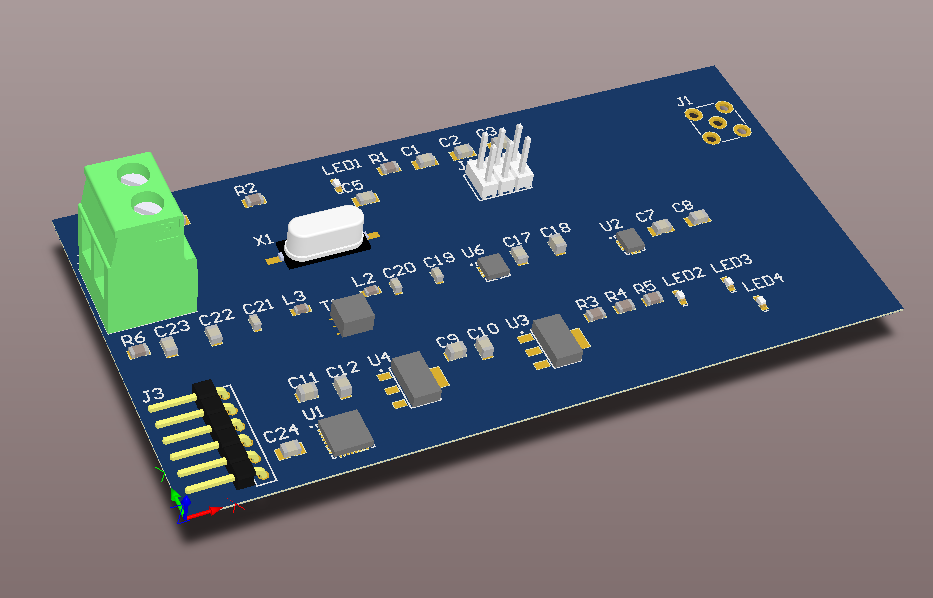
\includegraphics[width=\textwidth]{pcb.png}
    \caption{3D view of the designed PCB}
    \label{fig:pcb_3d}
\end{figure}

\end{document}
